This chapter lays out the theoretical background regarding the thesis's topic by first introducing the general concepts of a \emph{high-level language virtual machine} (HLL-VM) like the Java Virtual Machine (JVM) and then going on to more specific features of the GraalVM. In the following, the abstraction layer, the Truffle API is explained before coming to the explicit project Graal.js which is built on top of the Truffle language implementation framework. The last section discusses the ECMAScript parts of the topic with a brief glance at the current state of modules and what the proposal tries to achieve.

\section{High-Level language virtual machines}
A high-level language virtual machine (HLL-VM) is an abstraction layer relieving the programmer from several tasks with the main feature being platform independent development. When starting to discuss the platform independence it is foremost important to note why programs are usually platform bound. The main reason are two technologies which are presented in the next paragraph.

\subsection{Groundwork}
The following paragraphs serve as introduction into HLL-VMs and are based on the work of Smith in \cite{Smith} where the core ideas are bundled. Every computer employs some kind of \emph{instruction set architecture} (ISA) and an \emph{operating system} (OS). Every developed program is bound to these two technologies. If a program is developed for a particular pair of ISA/OS it has to be ported to run on a machine with a different pair of ISA/OS. The result of this paradigm is support overhead since every ported version of an application has to be updated individually. It is thus highly impractical to enforce such a development environment for every application program. By developing a HLL-VM this task is posed upon the development of the VM only and all other application programs being developed don't have to focus on platform dependency resulting in a more lean development and update process. Hence the VM delivers an abstraction layer for the ISA/OS couples and the applications running on top of the VM. \cite{Smith} 

How is the VM delivering the abstraction layer? High-level language virtual machines enhanced the concept of early VMs like \emph{P-code} \cite{pCode} by using virtual instruction set architectures (V-ISA) encompassing code and metadata, like data structures and resource-related information, independently of platforms. The code is simply interpreted the metadata loaded and thus turned into a machine-dependent version by the virtual machines provided emulator. \cite{Smith} This alone already stands out as a huge accomplishment but HLL-VMs come with even more features.

In today's computer landscape security risks can come from untrusted software run on machines. The HLL-VM, in particular the Java Virtual Machine (JVM),  provides a metaphoric sandbox in which the untrusted application can run without making the rest of the system outside of the VM vulnerable. Although it amplifies security there are loopholes to bypass said security measures especially when untrusted software is given explicit permission to go outside of the VM's provided resources. \cite{Smith, Lindholm} Hence running untrusted software is still not advised but made more secure with a HLL-VM. As said before security is not the only feature HLL-VMs serve. A feature directly improving code production is delivering an environment being beneficial for robust code. The details of the particular environment are subject to the upcoming discussion.

Especially when it comes to large-scale software systems robust code is key. Here the good fit of the object-oriented model and the platform independence make HLL-VMs the top technology in the field. How much a HLL-VM supports robustness is of course depending on the used VM but on the example of the Java Virtual Machine strong type-checking and garbage collection which will be explained later lift a lot of beverage off the programmer's shoulder making the programmer concentrate on the mere implementation and thus making code production more robust automatically because the execution environment is robust within itself. Additional merits of HLL-VMs come from technologies like dynamic linking saving network bandwidth or profiling for performance.\cite{Smith}

As the start of this subsection already stated a HLL-VM is an abstraction layer with a lot of features making a programmer's life considerably easier. This comes with some costs most notably performance. This cost is then highly reduced by certain techniques like the aforementioned profiling. With the groundwork laid out the next section discusses certain features of the Java Virtual Machine.

\subsection{The Java Virtual Machine}
The Java Virtual Machine (JVM) is, as its name states, developed around the language Java. Java is a general-purpose, object-oriented language with strong static types aimed as a production language. \cite{Gosling} Since one of the language's target is simplicity, details of machine representation are abstracted away from the user and not accessible through the language. This is in compliance with the points made in the HLL-VM chapter beforehand as the JVM serves as abstraction layer. First of the programmer does not have to worry about the ISA/OS-couple, secondly the aforementioned garbage collection abstracts machine representation as well. Further safety measures have been made like automatic storage management and checked array access. The Java sourcecode is usually compiled ahead of time (AOT) to \emph{Java bytecode} which is then run on the JVM. First of, what is java bytecode? Java bytecode is the instruction set of the JVM and is thus an intermediate form. Secondly, how and why is java bytecode created by AOT? Ahead of time compilation means that the programmed sourcecode gets compiled into a machine specific executable form. This form is, in the case of Java, Java bytecode, i.e. a class-file.\cite{Gosling} As stated before the JVM is the virtual sandbox environment in which an AOT-compiled java program, represented by the java bytecode, is executed. The JVM, like an actual machine, has an instruction set and access to various memory areas. With this in mind a JVM can also be directly implemented as a CPU or in various other direct ways. From knowing what the JVM is, the next paragraph dives deeper into the topic and explains how the JVM is constructed with the help of figure \ref{fig:jvm}.

As already explained the JVM executes Java bytecode which can be in the form of *.class-files. Before the thesis dives into the structure one note has to be made: The JVM is usually delivered as a Java Runtime Environment (JRE) or Java Development Kit (JDK). These include besides the Java Virtual Machine also the Java Application Programming Interface (API) classes. These are not directly part of the JVM but play a vital role in the simplification process for code production that is undertaken by the Java project. The next paragraph talks about some Java specifics before taking the topic towards JVM details.

\begin{figure}[h]
    \centering
	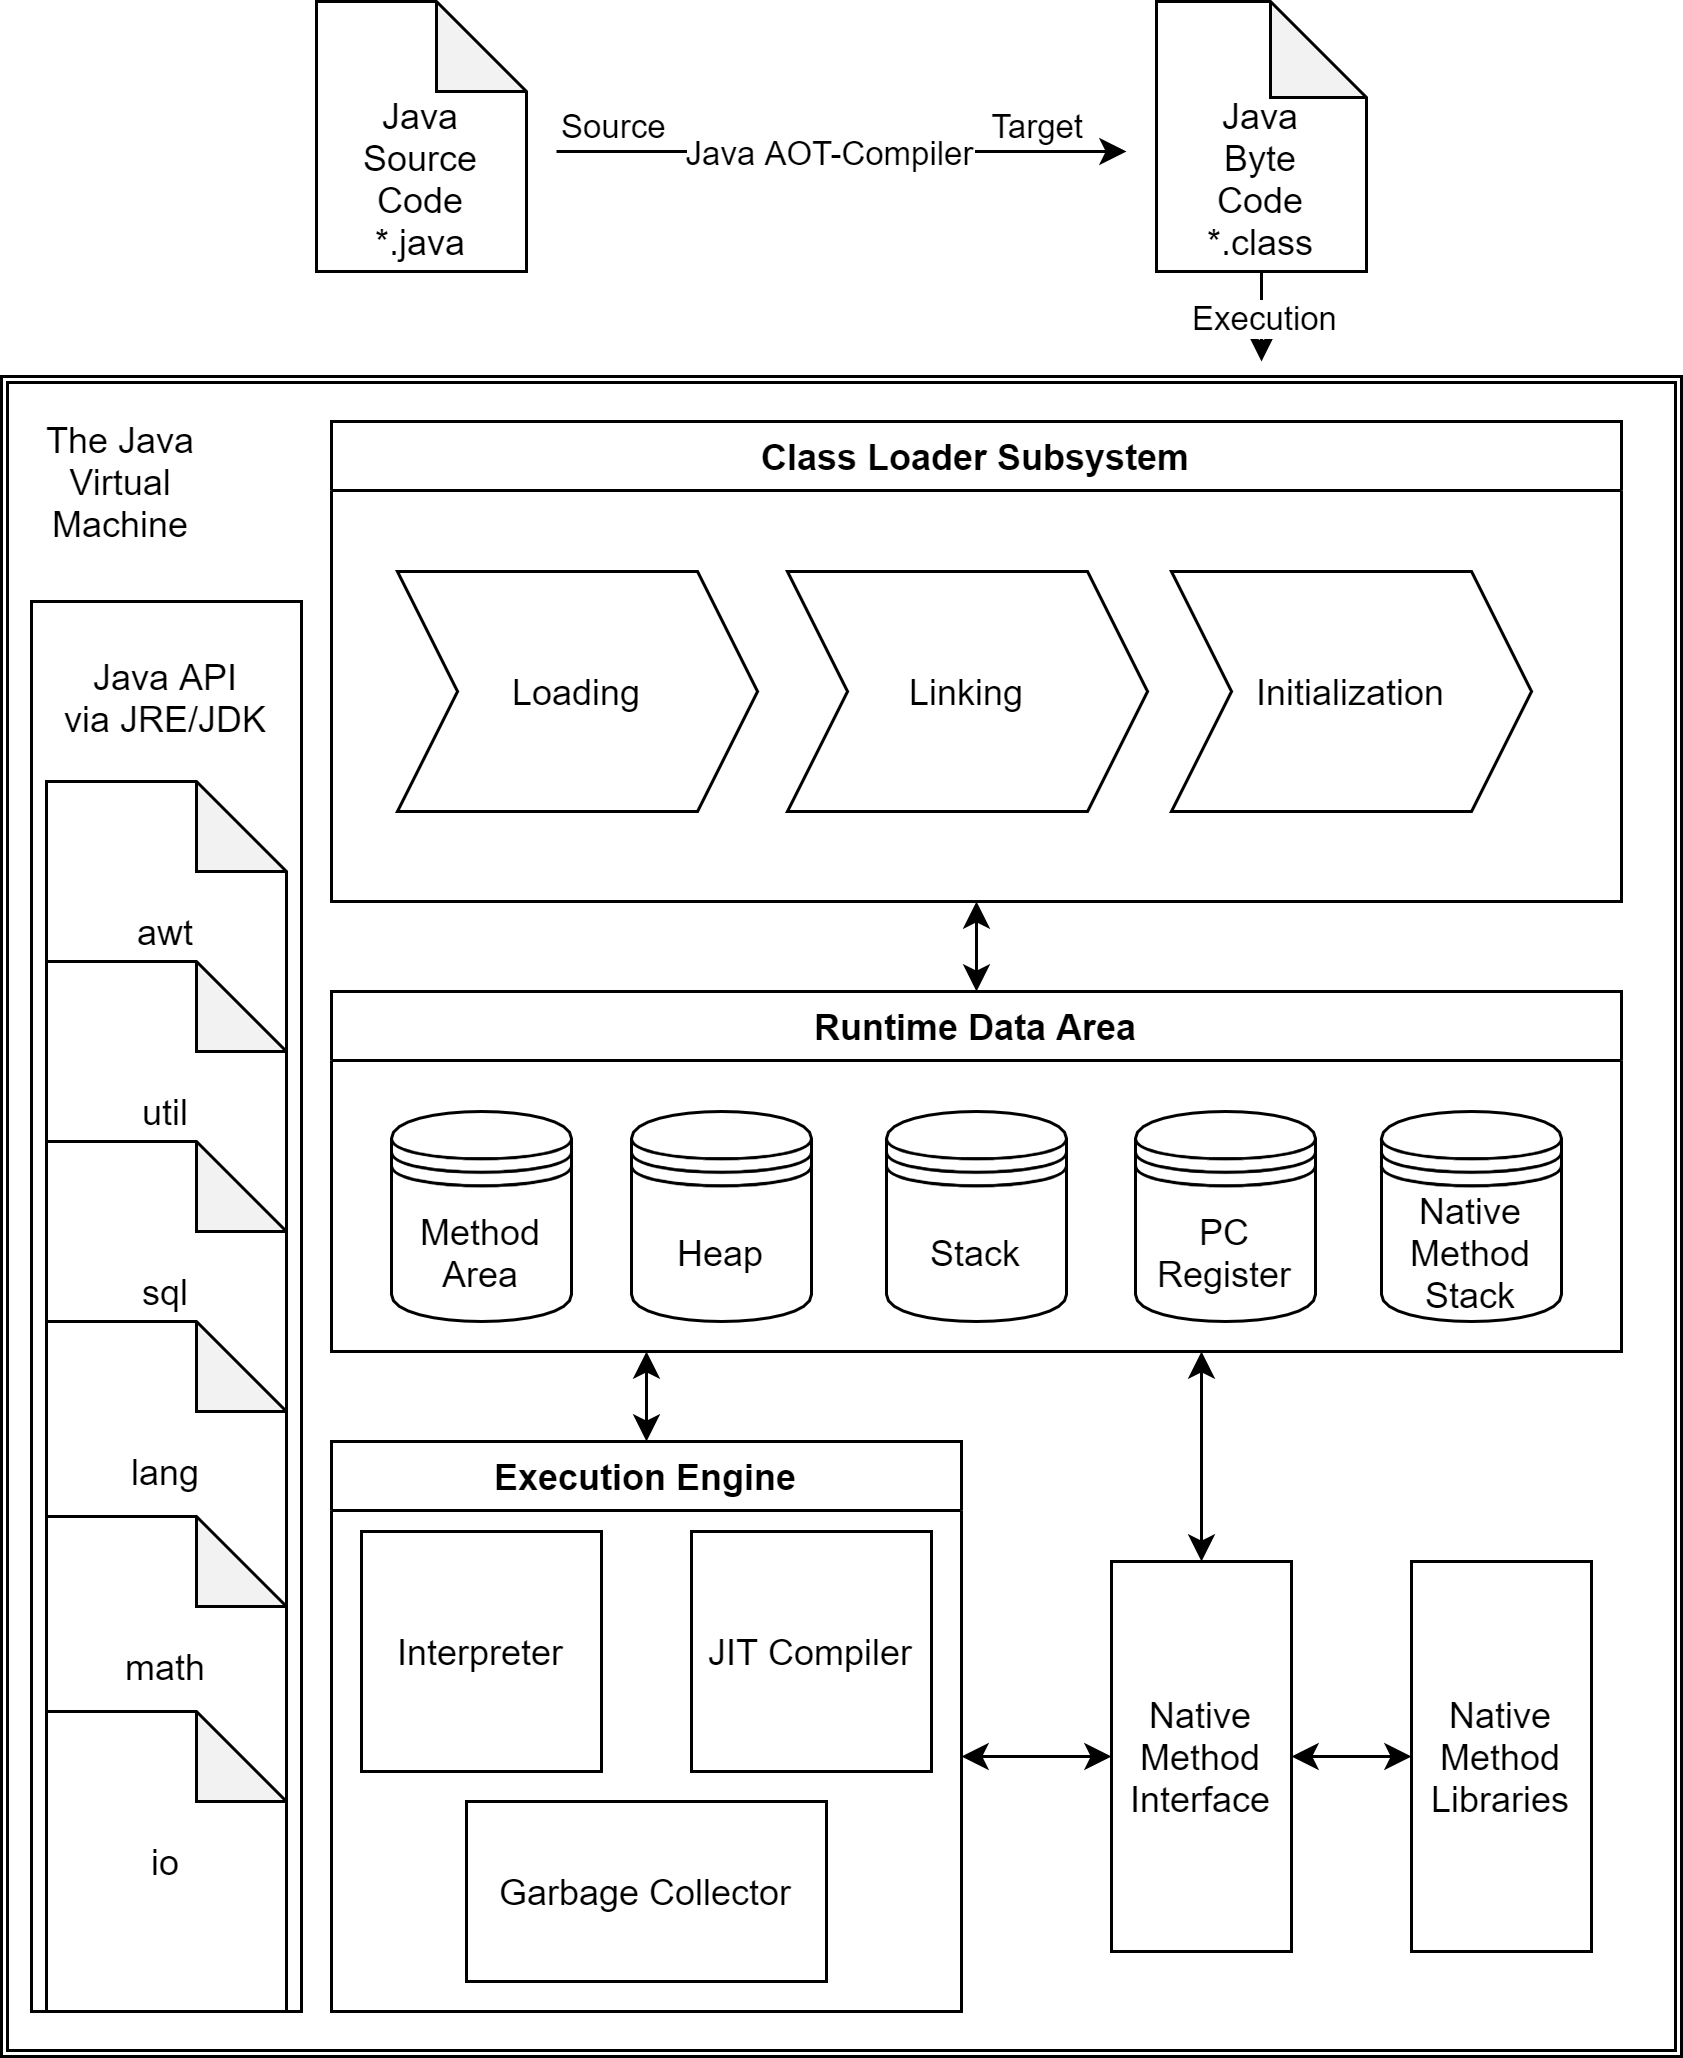
\includegraphics[scale=0.8]{figures/JVM.png}
	\caption{The Java Virtual Machine simplified structure}
	\label{fig:jvm}
\end{figure}

When talking about the JVM the mentioning of classes and interfaces is inevitable.
In further parts the distinction between class and interface is abbreviated as class.
Multiple causes for class creation exist. The class to be created can be referenced by the constant pool of another class or a class's method can be invoked via reflection.
The creation at the start of a program works via loading the initial class and initializing it and furthermore invoking the specified method \emph{public static void main(args[])}. The complete execution is driven by this method which, as soon as the program has more than this specific method and starting class, causes loading, linking and initialization of additional classes and invoking additional methods. \cite{Lindholm}

\subsubsection{Class Loader Subsystem}

When creating a class in execution the JVM transforms the implementation-independent bytecode into an implementation-specific internal representation of the class. Figure 2.1 shows how the sequential algorithm of loading, linking and initialization is conducted in the class loader subsystem.
The algorithm is executed step by step meaning that a class has to be completely loaded before linking can be started and it has to be verified and prepared to full extent before initialization. Again as can be seen in Figure 2.1 this process starts the execution process and is tightly knitted to the runtime data areas of the JVM.
The next paragraphs discuss the specifics of the three subcomponents and their tasks.

The loading is started by the class loader which can be the JVM bootstrap loader or a user-defined one. Before the JVM starts the class loader it checks whether the pair binary class name and class loader already exist in which case the class already exists thus eliminating the necessity of class creation. If creation proves necessary the class loader has to find the class' bytecode representation on the specific platform, usually a file with the class' name in a hierarchical filesystem. After finding, if not a specific error is thrown, the JVM parses the bytecode, which in turn might not produce a  valid outcome resulting in different kinds of errors. Optional superclasses may also have to be resolved. After these steps the pair of loader and class are saved by the JVM. Loading usually concerns the class itself however linking concerns its whole ecosystem. \cite{Lindholm}

The JVM links a class by preparing the class, superclasses, element type in case of array classes and resolving all symbolic references which as it is a recursive algorithm includes loading and linking these as well. The two strategies for resolution are an eager algorithm, meaning immediate loading and linking on verification, or loading and linking in a lazy way meaning resources are only loaded and linked when they are about to be used. Both have their respective advantages and disadvantages which won't be discussed in the scope of this thesis. At this point the JVM knows where the binary representation of a class can be found and which other classes are in the direct ecosystem of the class but the class's structure hasn't been checked yet. \cite{Lindholm}

Checking the class' structure is the main concern of the verification phase. In this step the class is checked for a static and structural constraints list. These include checks for appropriate type usage, number of arguments, instance initialization before usage, return types and many more. Any caught error in this step lead to ta thrown VerifyError. If no such error occurs the verification is finished and structural correctness of the binary class representation is acknowledged. \cite{Lindholm}

When doing the preparation of a class the JVM checks loading constraints on methods overriding those of superclasses and create and initialize static fields to default values. This phase can occur any time between creation and initialization but imperatively before initialization. Resolution in the context of the JVM means the process of dynamically determining conrete values from symbolic references in the run-time constant pool. The target of resolution includes classes, fields, methods, method types, method handles or dynamically computed constants. These different targets require different approaches, requiring class loading, lookup, etc. They can also fail and throw errors or succeed resulting in a resolved dynamic binding in the constant pool. With all these preceding steps the class is now ready for initialization.
Conceptually initializing a class is fairly simple as it is the mere execution of the initialization method. This can only be invoked by certain cases or instructions like \emph{new} or a subclass is initialized resulting in the initialization of the superclass. At this point the JVM's multithreading needs to be taken into account since synchronization is imperative. This again is solely handled by the JVM and of no concern for the application programmer. The concrete inner workings are generally spoken handled by object states and unique initialization locks. The Initialization phase is the final stage of the class loader subsystem. Now the different data areas are explained briefly. \cite{Lindholm}

\subsubsection{Runtime Data Area}

The JVM run-time data area is subdivided into five different data areas. These fulfill different tasks and are also different in their relation towards processes and threads as there are data areas being defined per thread and others per process. This results in some data areas existing as long as the JVM is running and some areas' existence being linked to their respective thread's existence. Areas that are shared by everything inside the JVM are JVM-defined structures, while thread specific data areas are called thread-defined structures. The data areas are, as can be seen in figure \ref{fig:jvm}, the method area, heap, stack, program counter register and the native method stack. The next paragraphs explain which area is responsible for which task and when they are created and destroyed.

The method area is shared between all JVM threads and is created on JVM start-up. It stores all per-class structures like the constant pool or fields and method data. Those are data every instance of a class shares analogous to each car having four tires.

The heap is a JVM-defined structure, as such is created on JVM start-up, and is shared between all threads. It is an allocation space for class instances and arrays on run-time. Allocation and deallocation in the JVM is automatically handled by the garbage collector which again can be shortly defined as an automatic storage management system. The structure of the heap is not necessarily contiguous and attributes like initial, maximum and minimum size can be defined by the programmer or user with so called command-line arguments that are given to the execution engine to take with the given program.

The stack is a thread-defined structure and is itself subdivided into thread-specific stacks. It does have a fixed size which is defined at stack creation. Regarding the data a stack holds: local variables, partial results and has its share in method invocation and return. The not necessarily contiguous stack is only changed by pushing and popping frames.

The program counter (PC) register holds the current program counters of all running threads and as such is a JVM-defined structure. A thread specific PC register contains the address of the thread-specific currently executed method.
The native method stack is an optional data area not supported by all JVMs. If it is supported it is similar to conventional stacks on a thread basis. They can be of fixed or dynamic size. These stacks fulfill a similar task to the regular stacks but are for code not written in Java. With the data areas explained the execution engine is the focus of the next few paragraphs.

\subsubsection{Execution Engine}

The execution engine is mainly built up of three different components, the interpreter, the just-in-time (JIT) compiler and the garbage collector as can be looked up in figure \ref{fig:jvm}. The interpreter is the part that executes the code directly/live including byte code getting translated to actual implementation-dependent machine code and its execution on the central processing unit (CPU) per instruction. This mechanism causes the interpreter to reinterpret, translate and execute the same code multiple times per instruction. This redundant interpreter pipeline work makes execution slow compared to AOT-compiled execution. When doing so the interpreter of the JVM profiles the run code for example by keeping track of how often a certain piece of code is executed. This profiling information is then used to choose the parts of code that get JIT-compiled hindering too many redundant interpretation steps.

A part of the byte code chosen for JIT-compilation is compiled to machine code and gets thus turned from implementation independent form into implementation dependent form. Afterwards if this part of the program gets executed again the machine code gets executed directly out from the cache where it's stored in the meantime. This method of choosing code hotspots that get executed often for compilation rather than continuous interpretation is called adaptive compilation and is used in the Oracle Hotspot VM. \cite{Lindholm}

The last component left out so far is the garbage collector (GC). It takes care of objects without references resulting them to be unreachable by application code. Such an object will be removed by GC and memory will be freed up. The GC is part of inner workings and fully functions without user interaction but the programmer can make a not guaranteed call for the GC.\cite{Lindholm} In programming languages like C a programmer would have to free memory explicitly. The obvious advantage is more direct control by the programmer but the disadvantage are possible memory leaks. The GC thus cares for memory and consequently robust code. A disadvantage of the GC is its appearance as a black box which means as a programmer you can't be sure at what point in execution unreachable resources are deleted. This concludes the JVM discussion with a wrap-up in the next paragraph.

This section explained the JVM ecosystem. It is split up between an AOT-compiler that creates Java bytecode out of Java source code and the runtime. From there on the JVM executes the bytecode. Generally speaking the JVM consists of three areas, the class loader subsystem, taking care of loading, linking and initialization, the runtime data area and the execution engine, consisting of the interpreter, the JIT compiler and garbage collector. Additionally to ease the programmer's work the JRE or JDK come with libraries. What hasn't been discussed in detail so far are technologies for making Java execute faster apart from features like hot spot profiling. These technologies are a core feature of GraalVM which is the topic of the next section.

\section{GraalVM}

As seen in the last two sections building a virtual machine for executing programming languages is a non-trivial task needing a lot of effort. A lot of this effort has to be redone for different programming languages. The core idea of GraalVM is to reduce this effort via a layered structure where each language implementation is in essence an abstract syntax tree (AST) interpreter via the Truffle API. All low level implementions like JIT compiling, data areas, memory management, optimizations and the like are reused by each language implementation connecting to the GraalVM or any JVM via Truffle. Considering performance these implementations are best run on top of GraalVM. Reasons for that are explained in the next section.

\begin{figure}[h!]
    \centering
    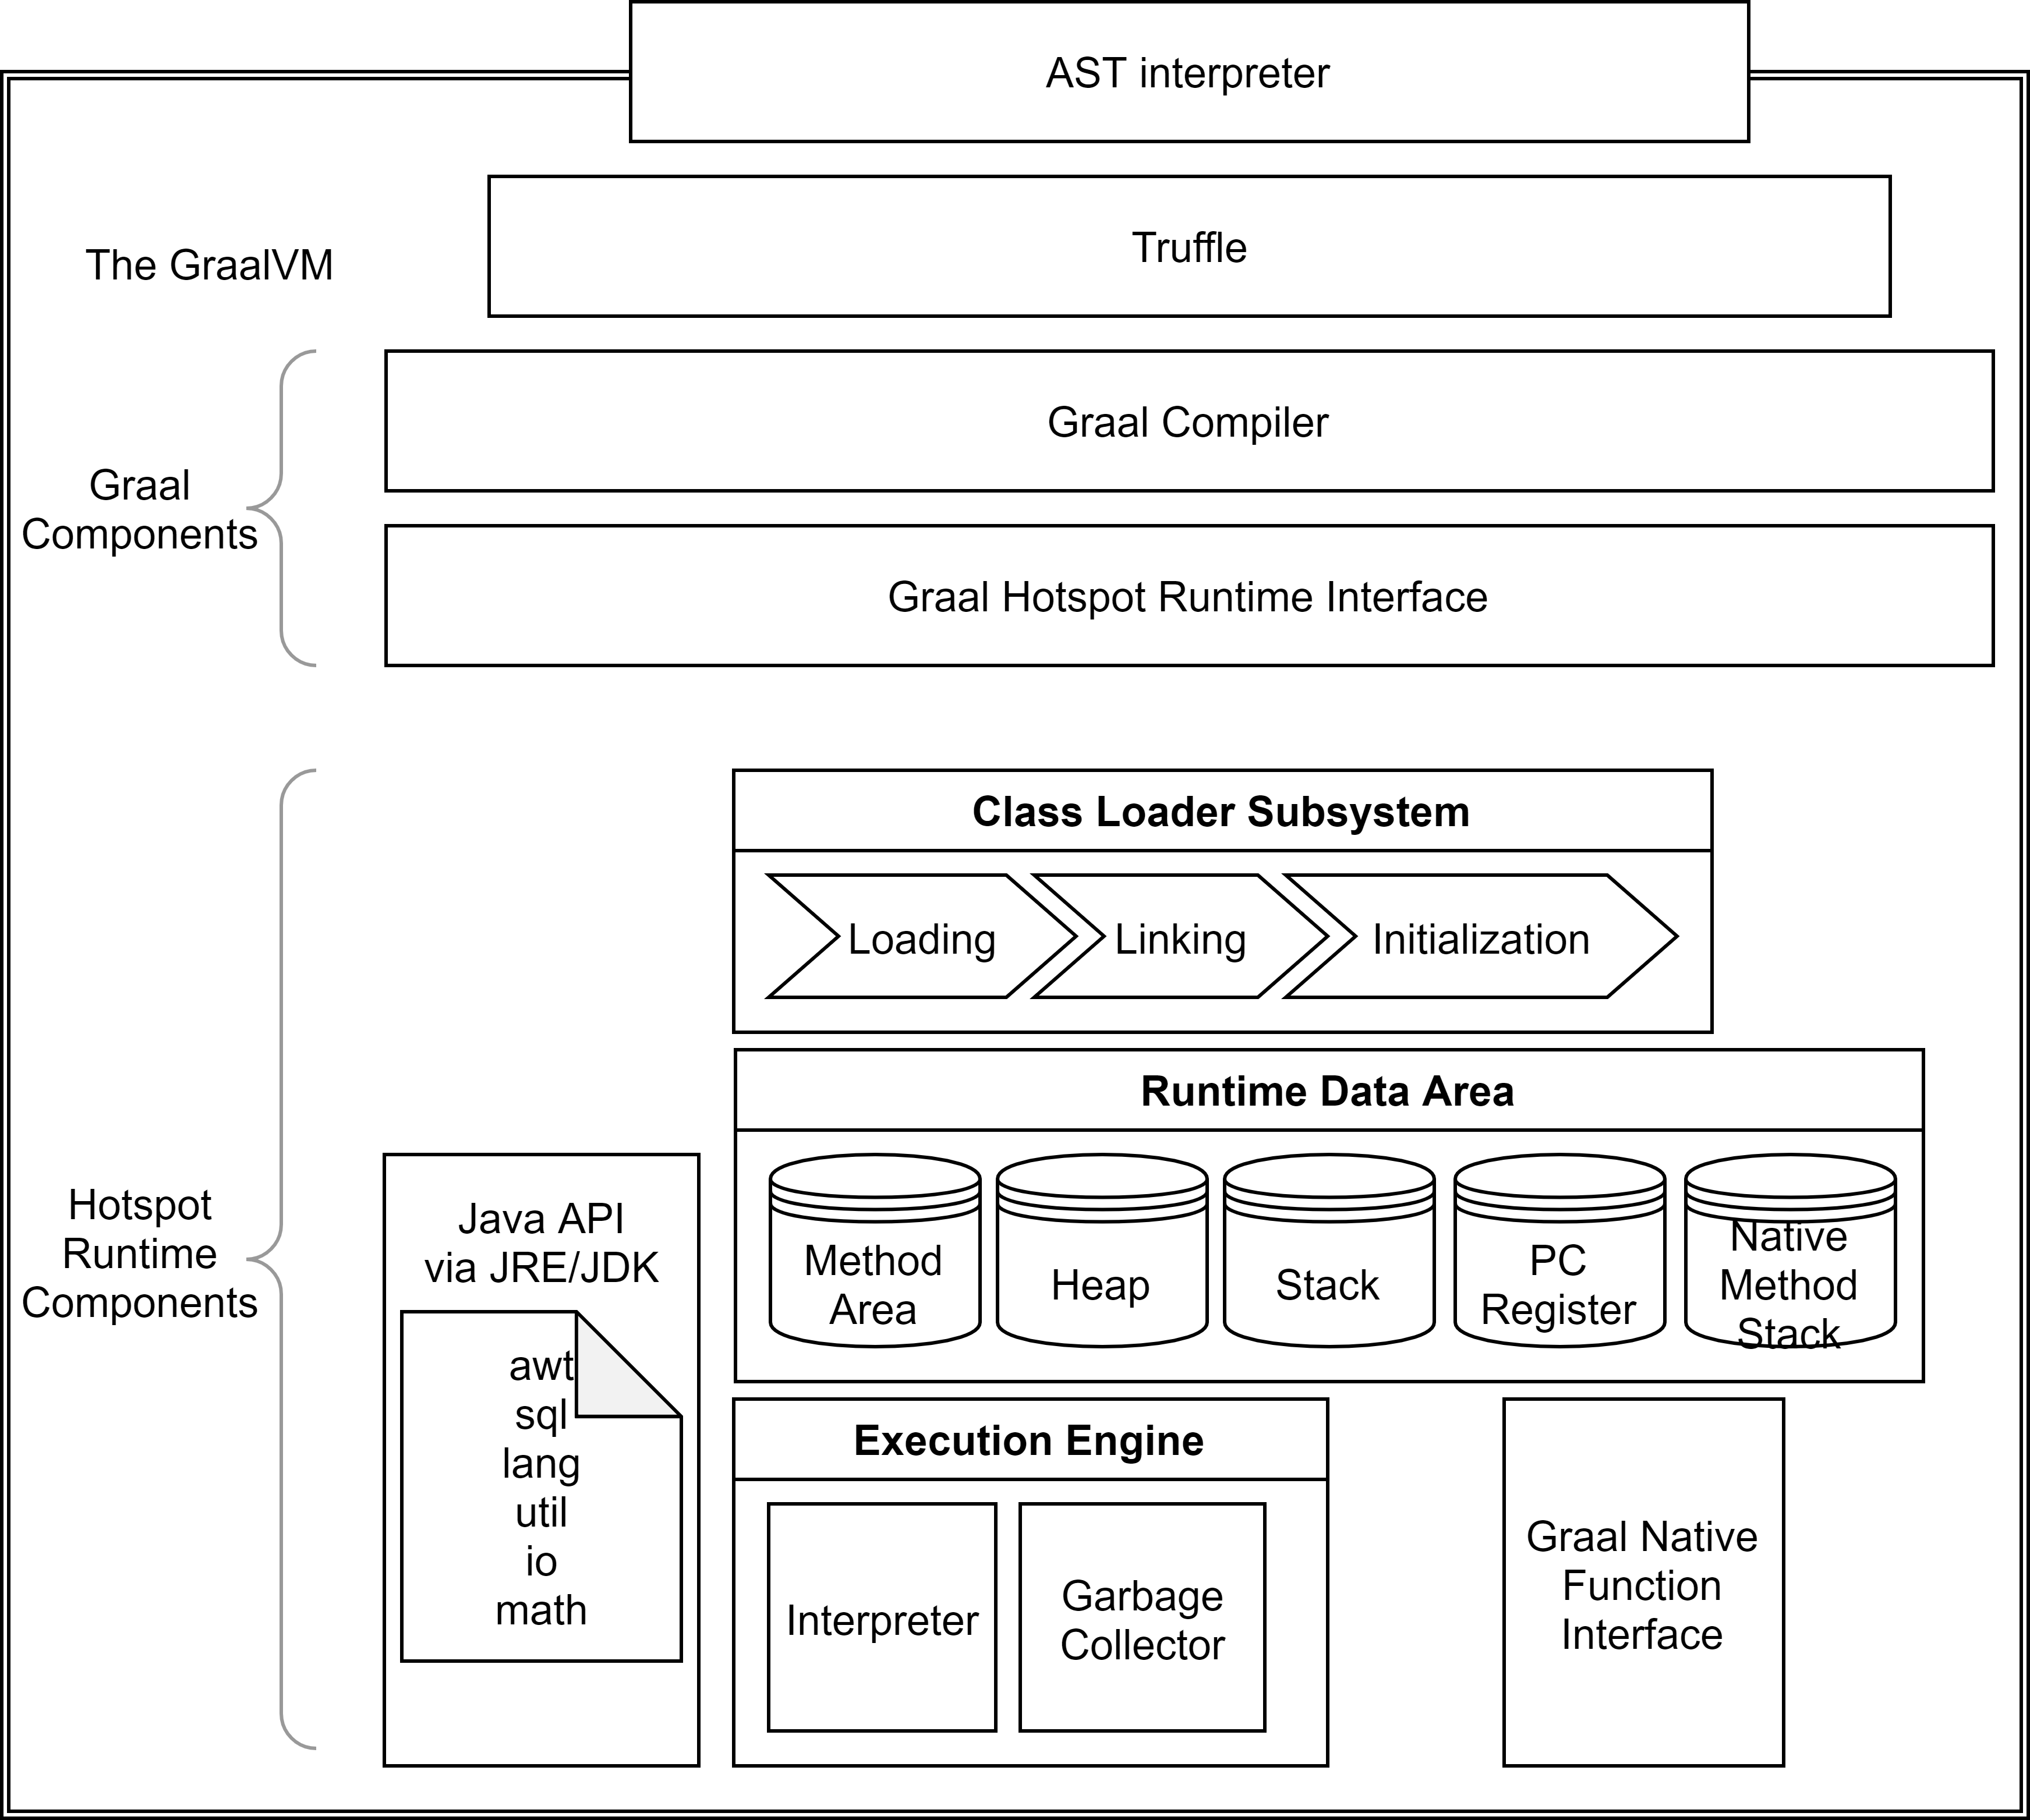
\includegraphics[scale=0.8]{figures/GraalVM.png}
    \caption{The Graal Virtual Machine simplified structure}
    \label{fig:graalvm}
\end{figure}

The GraalVM complete ecosystem is comprised of multiple technologies. In the runtime environment the GraalVM reuses most components from the HotSpot VM like the class loader subsystem, the runtime data area and parts of the execution engine, in particular the interpreter and the garbage collector, but replaces the HotSpot JIT compiler with the GraalVM compiler. Since the GraalVM compiler functions differently it also implements an interface between the regular HotSpot components and the GraalVM compiler. Outside of the VM it also has the Truffle framework for different language implementations. Already implemented languages are JavaScript, Ruby, R, python and LLVM-based languages like C, C++ and Rust. Thus the feature is able to end the segregation of programming languages. Another feature is its ability to be embedded in combination with OpenJDK, node.js or inside Oracle Database, while also being able to be run standalone. \cite{graalVMStart}
\subsection{GraalVM Compiler}\label{sec:graalcomp}
The GraalVM Compiler replaces the JIT compiler in a JRE. Other as the regular java JIT compiler it doesn't translate java bytecode directly to machine code but to the Graal IR. \cite{inproceedings} The Graal IR is a graph-based high-level intermediate representation. This intermediate representation is key to GraalVM's aggressive optimization techniques based on optimistic assumptions such as specific types and branch prediction. Aggressive optimization also means the compilation is prone to failures which are caught by so called guards. When a guard fails execution is transferred back to interpretation. This mechanism is called deoptimization. \cite{ChambDeopt} Compiled code gets saved as a VMs internal data structure and subsequent calls to the particular part of code get always directly executed in machine code omitting the unnecessary step of interpreting. Another component the GraalVM project substitutes is the Java Native Interface \cite{Lindholm}. It is exchanged with the Graal Native Function Interface (GNFI). \cite{grimmerNative} It allows for efficient native function calls within Java code.
\subsection{Truffle API}
The Truffle language implementation framework enables programmers to write an AST interpreter in Java for any programming language. The biggest advantage is the reuse of JVM runtime services such as automatic memory management with execution by a JVM. But how does the interpreter work?

The interpreter works by modeling language structures as nodes building the abstract syntax tree. Evaluation of the tree works by executing each node. Each node type shares basic specifics for executing their respective semantics. The whole tree gets then recursively evaluated by the recursive execute method calls.

\begin{figure}[h!]
    \centering
    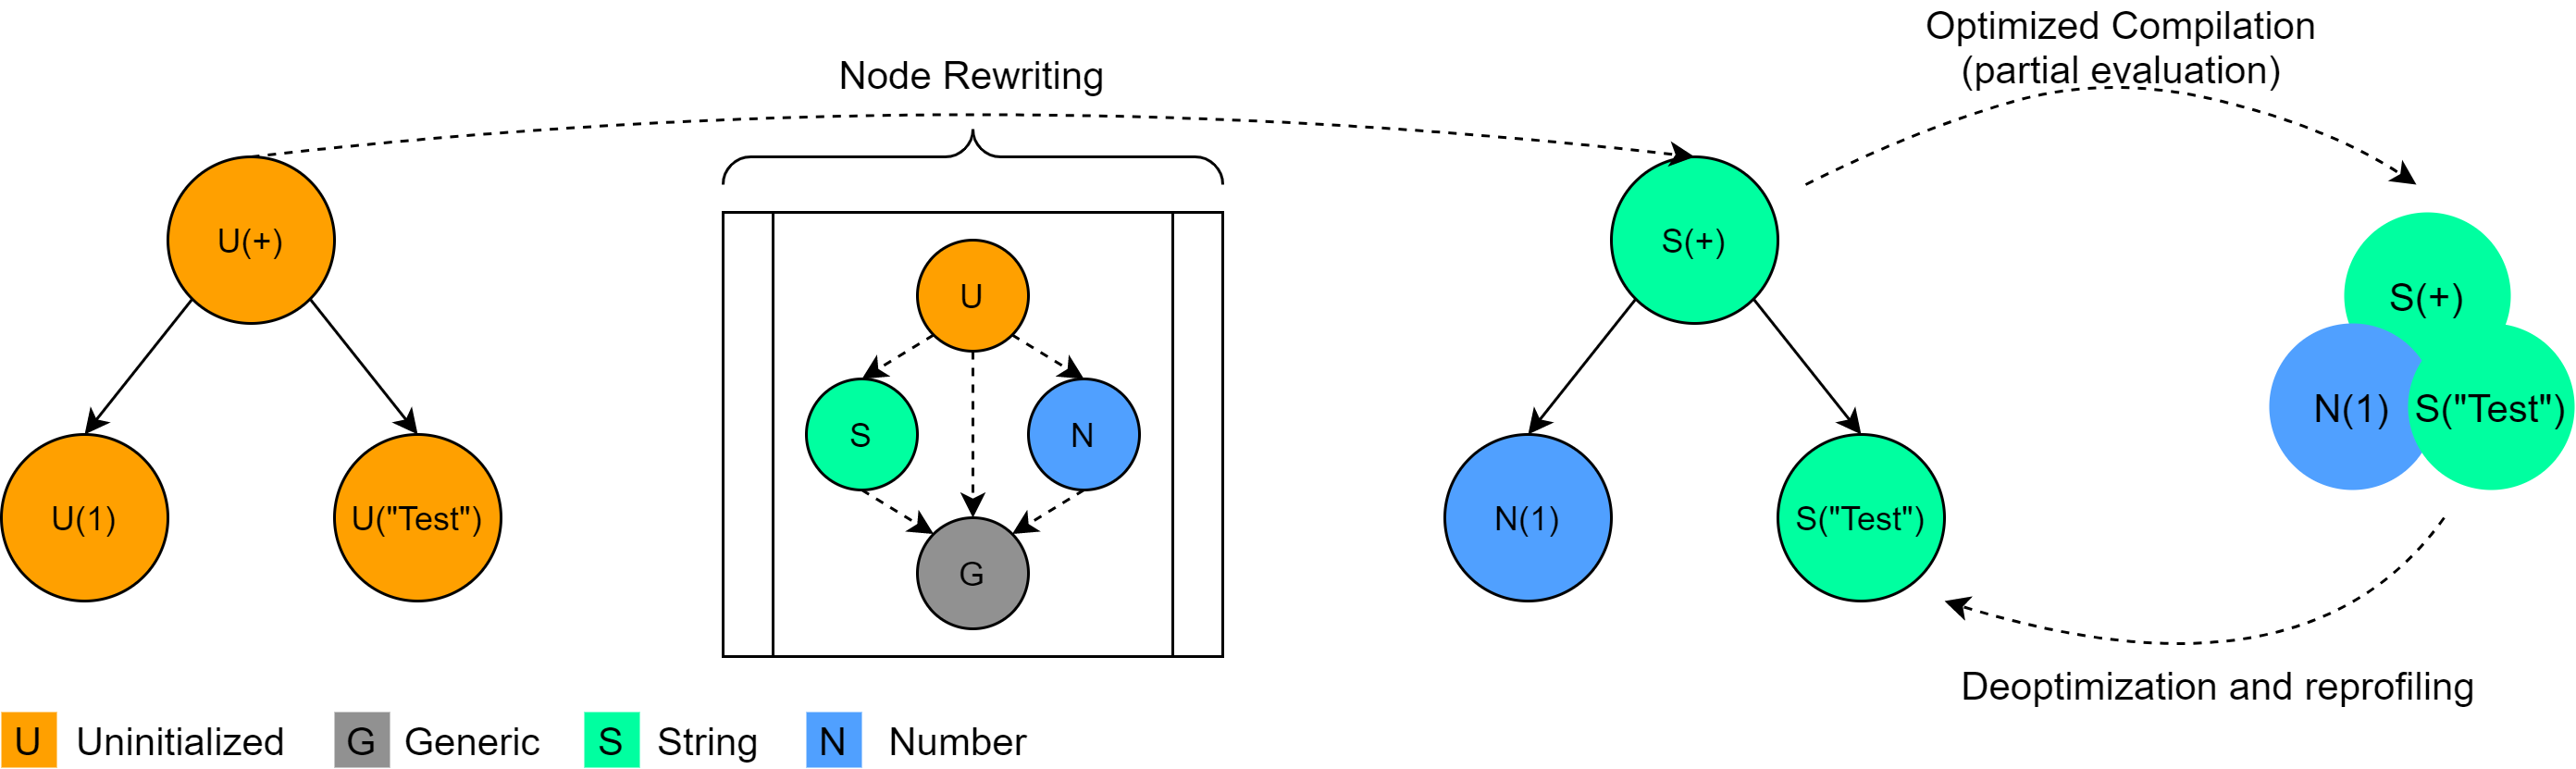
\includegraphics[scale=0.7]{figures/NodeJIT.png}
    \caption{Simplified Node Rewriting example}
    \label{fig:trufNR}
\end{figure}

Optimizations on AST level mostly work with speculative specialization techniques. On the left side of Figure \ref{fig:trufNR} the nodes are in an uninitialized state and write themselves into specialized variants at run time where profiling information is available. \cite{wuerthSelf} At that point execution happens in the interpreter. This specialized tree can then, after certain conditions are met, be compiled into what can be seen at the far right side of Figure \ref{:trufNR}. As we have discussed earlier in the GraalVM compiler speculative optimizations, like node specialization, are prone to failure. As soon as the compiled version's execution fails execution goes from the specialized compiled version back to a more generic version being interpreted and the cycle starts again. This cycle process is shown in the right side of Figure \ref{fig:trufNR}.
% The nodes rewrite themselves into specialized variants at run time where profiling information is available. \cite{wuerthSelf} As we have discussed earlier in the GraalVM compiler speculative optimizations, like node specialization, are prone to failure. Instead of going just back to interpretation a failed specialized Node rewrites itself back into a more generic version as can be seen in figure \ref{fig:trufNR}.  \cite{VMRule} What kind of specializations are possible via this approach?

What kind of specializations are possible via this approach? Type specialization especially with dynamic languages is an operation reducing code on runtime and thus creating speed up. To discuss this optimization method in more detail the add method with the + operator in the scripting language JavaScript is used. The add method in JavaScript is defined for various types including Strings and Numbers. We reduce the language's complexity to the aforementioned two types in the example. The example code in Listing \ref{lst:jsTypes} shows how addition in JavaScript works in different settings. The interpreter has to check the types of two operands from left to right before it can decide on which operation to use, an addition for numbers or one for strings. In line 1 a number and a string addition takes place, resulting in a string concatenation. In line 3 the interpreter takes the left plus as an integer plus, resulting in the addition of 1 and 2 to 3, while the second plus is interpreted as a string addition, leading again to a string concatenation. In line 5 the first plus is interpreted as a plus-sign, resulting in the string being parsed into a number which works in this case but not in the case of line 7. The second addition is a numeric one again in both lines.

\begin{lstlisting}[caption={JavaScript addition types minimal example}, label={lst:jsTypes}]
	var w = 1 + "Test" // results in "1Test"
	typeof(w) // string
	var x = 1 + 2 + "Test" // results in "3Test"
	typeof(x) // string
	var y = +"1" + 2 // results in 3
	typeof(y) // number
	var z = +"Test" + 1 // results in NaN
	typeof(z) // number
\end{lstlisting}

The node rewriting process shown in Figure \ref{fig:trufNR} happens at various states to achieve different goals. In the interpreter node rewriting is used to capture profiling feedback via runtime information such as the rate of node rewrites. If certain thresholds are surpassed the specialized AST gets compiled into machine code. If the execution fails the compiled code gets deoptimized back to the AST interpreter where again nodes are rewritten and now update the existing profile information. After this step the newly specialized AST gets compiled again. \cite{wuerthSelf}

One note on the compilation process: The compiler uses as said aggressive optimization methods. This operation is successful for stable ASTs. Then compilation techniques like method inlining and eliminating interpreter dispatch code can be performed. This technique is called partial evaluation.

In addition to type specialization truffle offers so called polymorphic inline caches. \cite{ChambOpti} An inline cache itself is simply caching a method from a former lookup at call site. In Truffle inline caches are built by chaining nodes which check for cached target matches which are then executed. At a predefined chain length the chain gets replaced by a polymorphic node handling all operations.

As discussed in the JVM section program loading often requires resolution. An implemented truffle language can cache resolved targets at run time by replacing an unresolved node with its resolved version. Thus further resolutions of this node are prevented which leads to an optimized version of the AST.

This section gave a small introduction into the Truffle API for implementing languages via an AST interpreter for running on top of a JVM and showed the optimizations that are conducted on AST level. After an AST at run time becomes stable with no more rewrites the AST is compiled dynamically to machine code. Truffle uses the JIT compiler of a JVM, in case of GraalVM the GraalVM compiler. If GraalVM is used the nodes' execute methods are inlined producing one compilation unit of the whole tree. In the next step the GraalVM compiler uses its aggressive optimization techniques for the whole inlined tree unit producing efficient machine code. These combined methods are based on the principle of the first Futamura Projection also called partial evaluation. \cite{FutaPart} As stated in section \ref{sec:graalcomp} guards or also optimization points need to be implemented to check all the assumptions made before compilation. As soon as it is necessary to rewrite a node during machine code execution the control flow gets transferred back to the interpreted AST to rewrite the node either on profiling information to another specialized version or a more generic version. \cite{ChambDeopt}

In conclusion the GraalVM project aims at simplifying language implementations and application programming while also trying to have a rapid run time. The simplification comes from introducing a framework for implementing languages as AST interpreters which can run on top of any JVM. The performance benefits are especially achieved from running the AST interpreter on top of the GraalVM which uses various techniques to bring run time performance to higher levels.
%\begin{tikzpicture}[nodes={draw, circle}, ->, minimum size=2cm, level distance = 2.5cm, sibling distance = 2.5cm]
%	\node[fill=lightorange] (p) {U(+)}
%		child { node[fill=lightorange] (n) {U(1)}}
%		child { node[fill=lightorange] (s) {U("Test")}};
%\end{tikzpicture}
%\begin{tikzpicture}[nodes={draw, circle}, ->, minimum size=2cm, level distance = 2.5cm, sibling distance = 2.5cm]
%\node[fill=lightgreen] (sp) {S(+)}
%child {node[fill=lightblue] (sn) {N(1)}}
%child {node[fill=lightgreen] (ss) {S("Test")}};
%\end{tikzpicture}\\ \\
%\begin{tikzpicture}[sibling distance=1cm]
%\node[fill=lightorange, label=right:{Uninitialized}] (u) {U};
%\node[below=.3cm of u,fill=lightblue, label=right:{Number}] (n) {N};
%\end{tikzpicture}
\section{Graal.js}
The Graal.js project is an AST interpreter on top of Truffle. It is in full compliance of the newest ECMAScript 2021 language specification \cite{kangax1, GraaljsComp} and growing support of the technical committee 39 (TC39) proposals for future ECMAScript language specifications. \cite{kangax2, gitTC}  The runtime can execute JavaScript and Node.js applications with the previous discussed benefits of the GraalVM technology stack. \cite{Graaljs} As a recap the most notable ones are performance and polyglot programming support with multithreading support.

\section{ECMAScript \& the current state of modules}
As stated in the introduction, in Chapter 1, ECMAScript is a script language that is the standard specification for JavaScript. The naming conflict originates from copyright issues with the name JavaScript being trademarked by SUN and ECMA being the organization on standardizing the language. \cite{10.1145/3386327} It is maintained by the ecma organization with the formalization process starting in 1996 resulting in the first ECMA-262 (ECMAScript specification) edition in 1997. Current state is the 12th edition with name EcmaScript 2021. \cite{ecma} The language is a multi-paradigm, dynamically typed, general-purpose scripting language with first-class functions. This means the language supports functional, imperative, reflective and object-oriented programming. The object-orientation is prototype-based meaning existing objects are used to reuse behavior. These design decisions were prone to blistering criticism in the past but still reside in the language. \cite{10.1145/3386327} A very specific language feature that hadn't been supported initially is the module.

With ECMAScript 6 the language included modules making it possible to divide code up into multiple files. Although this possibility has been around in JavaScript before, it was implemented by external libraries and not an inherently specified language feature. The ability to import modules as needed came with a rise in source code size in regular JavaScript programs. When the language started out it was not unusual to have a one-line \texttt{.js-}(JavaScript)file. As the code size grew the necessity of modules came with it which led to a multitude of concurring solutions. As script concatenation as the basic step meant manual building and testing, this method could only be used in simple projects while more difficult ones started using module loaders. Those in turn could also become complicated for larger code bases. To overcome these problems so called module bundlers, like Babel\footnote{https://babeljs.io/}, could be used to generate the needed JavaScript code at build time. Thus the code includes all dependencies in a single concatenated file. The specification of modules in ECMAScript bundled these efforts into one concept and gave implicit module support by the language. With this specification feature performance of module loading was pushed towards engine implementation.

In a short note to avert term mixup. ECMAScript is a language specification for script languages. The actual code written is in JavaScript and this language is then run via engines in browsers on computers. In hard terms the ECMAScript specification does not need to be fully supported by a particular browser and single features sometimes are left out but in general engine implementations follow the ECMAScript specification leading to the specification's features in JavaScript sourcecode.

In a broad sense modules at current state read like regular scripts with the difference of them being in strict-mode only and using imports and exports. The benefits are separate files with self-contained functionality, sharing of those files between different projects, diminishing naming conflicts and the robustness that comes with shared open source. But what are modules in the context of JavaScript in detail?

As a module is run in strict mode all declared variables, functions and classes are private and cannot be accessed from the outside. Only those top-level items that are explicitly exported by the keyword \emph{export} can be used from a script importing the module. This is then done by the keyword \emph{import} either the whole module or explicitly named items which can also be aliased.

As modules have to be loaded and are sometimes scattered throughout the web, deferring module loading is a default setting. Another note is the caching of modules. A module is only executed the first time it gets imported. All other scripts importing the module are given the already evaluated exports. This also means that a change in one of the exports is visible to all importing scripts.

This standard unfortunately left out the possibility to add inline modules into a script which results in modules just containing one exported function. This results into unnecessary files which could be avoided by inlining the module into the original script. This exact feature is discussed in Section 2.6.

\section{ECMAScript proposal process}
Before coming to module blocks themselves the general proposal process is to discussed in order to give insight at what development step the proposal resides at the time of this thesis. The ECMAScript proposal process \cite{ecmaProp} is split up in five stages from zero to four. The first notable stage is stage one where the general shape of the proposal has to be outlined with examples, problems and the shape of their solutions all collected in a public repository. At this stage the proposal is expected to undergo major changes. To be uplifted to stage two the proposal has to include an initial spec text with all major semantics and syntax but allowing placeholders. The stage is still expected to undergo certain changes but the general outline should be set. To reach stage three the proposal needs to have a finished and complete spec text that has been reviewed. In simple words the theoretic groundwork is finished and further improvements need empirical knowledge gathered on actual implementations. From this stage on the proposal is expected to undergo minimal change. The final stage before acceptance is stage four. Apart from a finished specification the proposal needs acceptance test in compliance with the rest of the ECMAScript tests and implementations that pass these tests as well as live experience by two VM implementations. \cite{ecmaProp} This concludes the proposal pipeline discussion which serves as a state overview for the upcoming proposal module blocks.

\section{Proposal: Module blocks}
Module blocks are an official TC39 proposal from Daniel Ehrenberg and Surma at stage 2 as of July 2021. \cite{gitMB} As stated ECMAScript does not have the feature of inlining modules. This causes several issues in programming applications, most notably code composition and file count but also CSP (Content Security Policy). In the current specified state if code should be run in parallel an additional file is needed resulting in every Worker (node.js feature) needing a separate file. So module blocks work like a module but are inside the script where they are also imported. One important note to take is the non closure of module blocks following the principle of coding in one place, running it anywhere. It can thus also be imported from any Realm and is code independent of a particular context. So in a sense module blocks are mainly a syntactical addition to ECMAScript as the concept is to provide a syntax for inlined module contents as can be seen by Figure \ref{fig:mbSyn}. \cite{gitMB, ecma} These can then afterwards be imported asynchronously. Reason being the ability of module blocks to import other modules as well. As regular modules since ES6 module blocks will be cached in the module map after the first import. One note to take is, that module blocks need to be imported via dynamic \texttt{import()} calls rather than import statements. This is due to them not being addressable as specifier strings. Dynamic import  has a particular positive impact on performance as module blocks will only be loaded on a base of need.

\begin{figure}[h!]
    \centering
    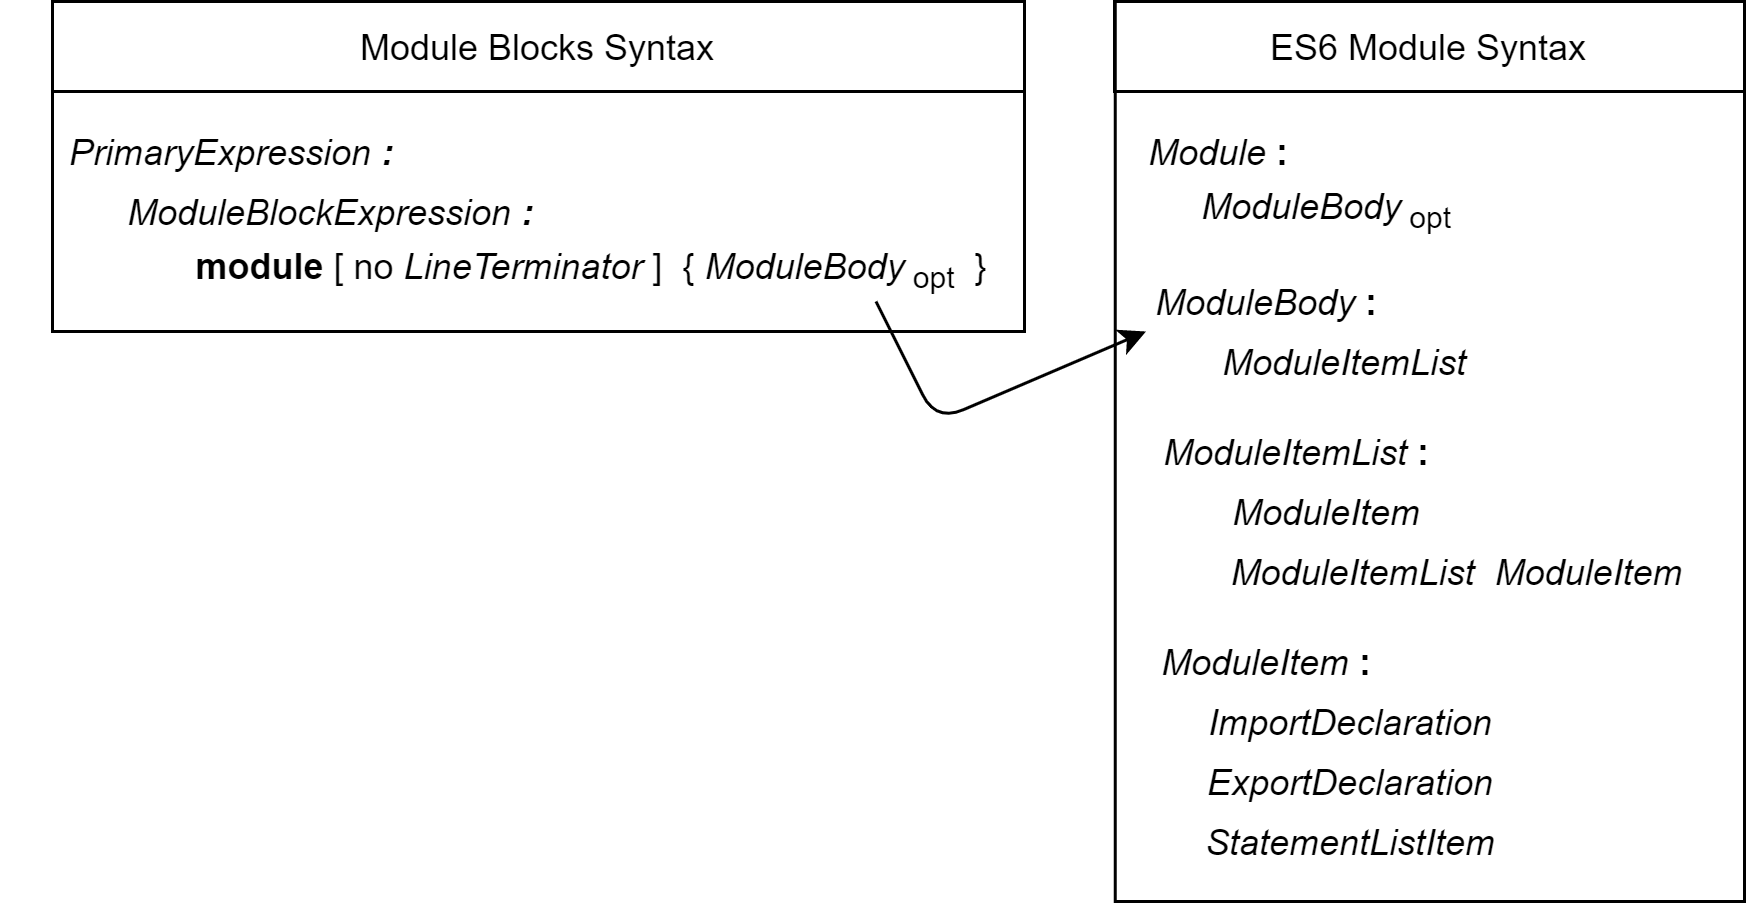
\includegraphics[scale=0.165]{figures/ModuleSyntax.png}
    \caption{Syntax of Module Blocks and ES6 Modules}
    \label{fig:mbSyn}
\end{figure}

%The whole module loading process can be pictured as a graph and as ModuleBlocks are only imported via dynamic import this creates a second graph. Hence the ModuleBlock's module references are processed separately from the referencing module.